\documentclass[12pt,letterpaper]{exam}
\usepackage[lmargin=1in,rmargin=1in,tmargin=1in,bmargin=1in]{geometry}
\usepackage{../style/exams}

% -------------------
% Course & Exam Information
% -------------------
\newcommand{\course}{MAT 108: Exam 3}
\renewcommand{\term}{Fall -- 2022}
\newcommand{\examdate}{12/15/2022}
\newcommand{\timelimit}{85 Minutes}

\setbool{hideans}{false} % Student: True; Instructor: False

% -------------------
% Content
% -------------------
\begin{document}

\examtitle
\instructions{Write your name on the appropriate line on the exam cover sheet. This exam contains \numpages\ pages (including this cover page) and \numquestions\ questions. Check that you have every page of the exam. Answer the questions in the spaces provided on the question sheets. Be sure to answer every part of each question and show all your work. If you run out of room for an answer, continue on the back of the page --- being sure to indicate the problem number.} 
\scores
\bottomline
\newpage

% ---------
% Questions
% ---------
\begin{questions}

% Question 1
\newpage
\question[10] Define the following vectors:
	\[
	\mathbf{u}= \begin{pmatrix} 2 \\ -1 \\ 0 \\ -3 \end{pmatrix} \qquad
	\mathbf{v}= \begin{pmatrix} 5 \\ 2 \\ -1 \\ 4 \end{pmatrix}
	\]
Showing all your work, compute the following:
	\begin{enumerate}[(a)]
	\item $-3 \mathbf{u}$
	\item $\mathbf{v} - \mathbf{u}$
	\item $\mathbf{u} \cdot \mathbf{v}$
	\end{enumerate} \pspace

\sol 
\begin{enumerate}[(a)]
\item 
	\[
	-3 \mathbf{u}= -3 \begin{pmatrix} 2 \\ -1 \\ 0 \\ -3 \end{pmatrix}= \begin{pmatrix} -3 \cdot 2 \\ -3 \cdot -1 \\ -3 \cdot 0 \\ -3 \cdot -3 \end{pmatrix}= \begin{pmatrix} -6 \\ 3 \\ 0 \\ 9 \end{pmatrix}
	\] \pspace

\item 
	\[
	\mathbf{v} - \mathbf{u}= \begin{pmatrix} 5 \\ 2 \\ -1 \\ 4 \end{pmatrix} - \begin{pmatrix} 2 \\ -1 \\ 0 \\ -3 \end{pmatrix}= \begin{pmatrix} 5 - 2 \\ 2 - (-1) \\ -1 - 0 \\ 4 - (-3) \end{pmatrix}= \begin{pmatrix} 3 \\ 3 \\ -1 \\ 7 \end{pmatrix}
	\] \pspace

\item 
	\[
	\mathbf{u} \cdot \mathbf{v}= \begin{pmatrix} 2 \\ -1 \\ 0 \\ -3 \end{pmatrix} \cdot \begin{pmatrix} 5 \\ 2 \\ -1 \\ 4 \end{pmatrix}= 2(5) + (-1)2 + 0(-1) + (-3)4= 10 - 2 + 0 - 12= -4
	\]
\end{enumerate}



% Question 2
\newpage
\question[10] Define the following matrices:
	\[
	A= \begin{pmatrix} 1 & -1 \\ 0 & 4 \end{pmatrix} \qquad
	B= \begin{pmatrix} -2 & 0 & 1 \\ 3 & -1 & 5 \end{pmatrix} \qquad
	C= \begin{pmatrix} 6 & 1 \\ -2 & 3 \end{pmatrix}
	\]

\begin{enumerate}[(a)]
\item Compute $B^T$.
\item Showing all your work, compute $5A$.
\item Showing all your work, compute $A - C$.
\item Only one of the possible matrix products $AB$ and $BA$ is defined. For the one which is defined, showing all your work, compute that product. 
\end{enumerate} \pspace

\sol 
\begin{enumerate}[(a)]
\item 
	\[
	B^T= \begin{pmatrix} -2 & 0 & 1 \\ 3 & -1 & 5 \end{pmatrix}^T= \begin{pmatrix} -2 & 3 \\ 0 & -1 \\ 1 & 5 \end{pmatrix}
	\] \pspace

\item 
	\[
	5A= 5\begin{pmatrix} 1 & -1 \\ 0 & 4 \end{pmatrix}= \begin{pmatrix} 5 \cdot 1 & 5 \cdot -1 \\ 5 \cdot 0 & 5 \cdot 4 \end{pmatrix}= \begin{pmatrix} 5 & -5 \\ 0 & 20 \end{pmatrix}
	\] \pspace

\item 
	\[
	A - C= \begin{pmatrix} 1 & -1 \\ 0 & 4 \end{pmatrix} - \begin{pmatrix} 6 & 1 \\ -2 & 3 \end{pmatrix}= \begin{pmatrix} 1 - 6 & -1 - 1 \\ 0 - (-2) & 4 - 3 \end{pmatrix}= \begin{pmatrix} -5 & -2 \\ 2 & 1 \end{pmatrix}
	\] \pspace

\item If $GH$ are $m \times n$ and $r \times s$ matrices, respectively, then $GH$ is defined if and only if $n= r$. If so, the product $GH$ is a $m \times s$ matrix. The matrix $A$ is $2 \times 2$ and $B$ is $2 \times 3$. Because $3 \neq 2$, the product $BA$ is not defined. However, because $2= 2$, the product $AB$ is defined. Furthermore, $AB$ is a $2 \times 3$ matrix. We have\dots
	\[
	\begin{aligned}
	AB&= \begin{pmatrix} 1 & -1 \\ 0 & 4 \end{pmatrix} \begin{pmatrix} -2 & 0 & 1 \\ 3 & -1 & 5 \end{pmatrix} \\[0.3cm]
	&= \begin{pmatrix}1(-2) + (-1)3 & 1(0) + (-1)(-1) & 1(1) + (-1)5 \\ 0(-2) + 4(3) & 0(0) + 4(-1) & 0(1) + 4(5) \end{pmatrix} \\[0.3cm]
	&= \begin{pmatrix} -2 - 3 & 0 + 1 & 1 - 5 \\ 0 + 12 & 0 - 4 & 0 + 20 \end{pmatrix} \\[0.3cm]
	&= \begin{pmatrix} -5 & 1 & -4 \\ 12 & -4 & 20 \end{pmatrix}
	\end{aligned}
	\]
\end{enumerate}



% Question 3
\newpage
\question[10] Consider the following system of linear equations:
	\[
	\begin{aligned}
	5x_1 - 3x_2 + 4x_3 - x_4= 12 \\
	x_1 + 10x_2 + 9x_4= 10 \\
	6x_1 - x_2 + 2x_3 + x_4= -6
	\end{aligned}
	\]

\begin{enumerate}[(a)]
\item Find the coefficient matrix for this system of equations. 
\item Find the constant vector for this system of equations.
\item Find the augmented matrix for this system of equations. 
\end{enumerate} \pspace

\sol We order the variables $x_1, x_2, x_3, x_4$. We make sure each variable is present and in this order in each equation. This gives us\dots
	\[
	\begin{aligned}
	5x_1 - 3x_2 + 4x_3 - x_4= 12 \\
	x_1 + 10x_2 + 0x_3 + 9x_4= 10 \\
	6x_1 - x_2 + 2x_3 + x_4= -6
	\end{aligned}
	\]

\begin{enumerate}[(a)]
\item The coefficient matrix is\dots
	\[
	\begin{pmatrix}
	5 & -3 & 4 & -1 \\
	1 & 10 & 0 & 9 \\
	6 & -1 & 2 & 1
	\end{pmatrix}
	\] \pspace

\item The constant vector is\dots
	\[
	\begin{pmatrix} 12 \\ 10 \\ -6 \end{pmatrix}
	\] \pspace

\item The augmented matrix is\dots
	\[
	\begin{pmatrix}
	5 & -3 & 4 & -1 & 12 \\
	1 & 10 & 0 & 9 & 10 \\
	6 & -1 & 2 & 1 & -6
	\end{pmatrix}
	\]
\end{enumerate}



% Question 4
\newpage
\question[10] Below is an augmented matrix corresponding to a system of linear equations in reduced-row echelon form. If there were solution(s) to the system of equations, find them. If not, explain why. 
	\[
	\begin{pmatrix}
	1 & 0 & 0 & 5 \\
	0 & 1 & 0 & -6 \\
	0 & 0 & 1 & 7
	\end{pmatrix}	
	\] \pspace

\sol Each of the columns of the matrix corresponds to a variable---except for the last column which corresponds to the `other' side of the equalities. There are then $4 - 1= 3$~variables. Writing out the equalities corresponding to each row, we have\dots

Observe that the last row tells us that\dots
	\[
	\begin{gathered}
	1x_1 + 0x_2 + 0x_3= 5 \\
	0x_1 + 1x_2 + 0x_3= -6 \\
	0x_1 + 0x_2 + 1x_3= 7
	\end{gathered}
	\]
But this immediately yields:
	\[
	\begin{cases}
	x_1= 5 \\
	x_2= -6 \\
	x_3= 7
	\end{cases}
	\]
Therefore, there is a unique solution: $(x_1, x_2, x_3)= (5, -6, 7)$.  



% Question 5
\newpage
\question[10] Below is an augmented matrix corresponding to a system of linear equations in reduced-row echelon form. If there were solution(s) to the system of equations, find them. If not, explain why. 
	\[
	\begin{pmatrix}
	1 & 0 & 0 & 0 & 6 \\
	0 & 1 & 0 & 0 & 1 \\
	0 & 0 & 1 & 0 & -4 \\
	0 & 0 & 0 & 0 & 1 
	\end{pmatrix}	
	\] \pspace

\sol Each of the columns of the matrix corresponds to a variable---except for the last column which corresponds to the `other' side of the equalities. There are then $5 - 1= 4$~variables. Writing out the equality corresponding to the last row, we have\dots
	\[
	\begin{gathered}
	0x_1 + 0x_2 + 0x_3 + 0x_4= 1 \\
	0= 1
	\end{gathered}
	\]
This is obviously impossible. Therefore, the original system of equalities was inconsistent, i.e. there is no solution to the original system of equations. 



% Question 6
\newpage
\question[10] Below is an augmented matrix corresponding to a system of linear equations in reduced-row echelon form. If there were solution(s) to the system of equations, find them. If not, explain why. 
	\[
	\begin{pmatrix}
	1 & 0 & 0 & -5 \\
	0 & 1 & -3 & 8 \\
	0 & 0 & 0 & 0
	\end{pmatrix}	
	\] \pspace

\sol Each of the columns of the matrix corresponds to a variable---except for the last column which corresponds to the `other' side of the equalities. There are then $4 - 1= 3$~variables. We mark the pivot columns of the matrix: 
	\[
	\begin{pmatrix}
	\boxed{1} & 0 & 0 & -5 \\
	0 & \boxed{1} & -3 & 8 \\
	0 & 0 & 0 & 0
	\end{pmatrix}	
	\]
Therefore, $x_1$ and $x_2$ will be `fixed.' We then take $x_3$ to be a free variable. The first row gives us the equality $1x_1 + 0x_2 + 0x_3= -5$, i.e. $x_1= -5$. The second row gives us the equality $0x_1 + 1x_2 - 3x_3= 8$, i.e. $x_2 - 3x_3= 8$. Solving for $x_2$ yields $x_2= 3x_3 + 8$. Therefore, there are infinitely many solutions, all of the form:
	\[
	\begin{cases}
	x_1= -5 \\
	x_2= 3x_3 + 8 \\
	x_3 \colon \text{free}
	\end{cases}
	\]



% Question 7
\newpage
\question[10] Consider the feasible set given below:
	\[
	\fbox{
	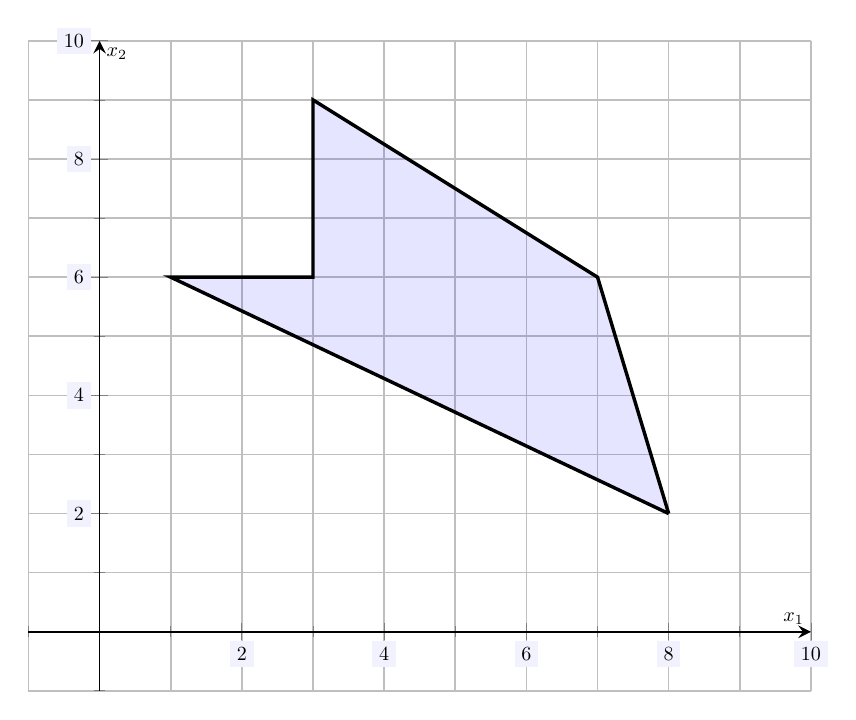
\begin{tikzpicture}[scale=1.45,every node/.style={scale=0.5}]
	\begin{axis}[
	grid=both,
	axis lines=middle,
	ticklabel style={fill=blue!5!white},
	xmin= -1, xmax=10,
	ymin= -1, ymax=10,
	xtick={0,2,4,6,8,10},
	ytick={0,2,4,6,8,10},
	minor tick = {-1,0,1,...,10},
	xlabel=\(x_1\),ylabel=\(x_2\),
	]
	\draw[line width=0.01cm,fill= blue,opacity=0.1] (8,2) -- (7,6) -- (3,9) -- (3,6) -- (1,6) -- (8,2);
	\draw[line width=0.03cm] (8,2) -- (7,6) -- (3,9) -- (3,6) -- (1,6) -- (8,2);
	\end{axis}
	\end{tikzpicture}
	}
	\]
Fully explaining your reasoning and showing all your work, find the maximum and minimum value of $z= 6x_1 - 5x_2$ on this feasible set. \pspace

\sol The function $z= 6x_1 - 5x_2$ is linear in $x_1, x_2$. The feasible set shown above is bounded and nonempty. Therefore, the Fundamental Theorem of Linear Programming states that the maximum and minimum values of $z$ exist and occur at a corner point for the region. We then simply evaluate $z$ at each of the corner points for the region: \par
	\begin{table}[ht]
	\centering
	\begin{tabular}{cl}
	Corner Point & $z= 6x_1 - 5x_2$ \\ \hline
	$(1, 6)$ & $z= 6(1) - 5(6)= 6 - 30= -24$ \\
	$(3, 6)$ & $z= 6(3) - 5(6)= 18 - 30= -12$ \\
	$(3, 7)$ & $z= 6(3) - 5(7)= 18 - 35= -17$ \\
	$(7, 6)$ & $z= 6(7) - 5(6)= 42 - 30= 12$ \\
	$(8, 2)$ & $z= 6(8) - 5(2)= 48 - 10= 38$
	\end{tabular}
	\end{table} \par
Therefore, the minimum value for $z$ on this region is $-24$ and occurs at $(1, 6)$ and the maximum value for $z$ on this region is $38$ and occurs at $(8, 2)$. 
	\[
	\boxed{
	\begin{gathered}
	\min z= -24 \text{ at } (1, 6) \\
	\max z= 38 \text{ at } (8, 2)
	\end{gathered}
	}
	\]

	

% Question 8
\newpage
\question[10] Find the initial simplex tableau corresponding to the maximization problem shown below:
	\[
	\begin{aligned}
	\max z= 4.3x_1 \,+ &\,5.7x_2 - 7.1x_3 - 5.6 x_4 \\
	6.9x_1 - 3.3x_2 &+ 7.9x_4 \leq 10.3 \\
	2.4x_1 - 5.8x_2 &+ 7.3x_3 \leq 14.3 \\
	8.4x_1 - 9.2x_2 \,+\, &1.8x_3 - 3.1x_4 \geq -10.8 \\
	x_1, x_2, &\, x_3, x_4 \geq 0
	\end{aligned}
	\] \pspace

\sol We need all inequalities to have a nonnegative number on the `right side' of the inequality. So we must multiply both sides of the third inequality by $-1$, so that we obtain the following inequalities (ignoring the non-negativity inequalities): 
	\[
	\begin{cases}
	6.9x_1 - 3.3x_2 + 0x_3 + 7.9x_4 \leq 10.3 \\
	2.4x_1 - 5.8x_2 + 7.3x_3 + 0x_4 \leq 14.3 \\
	-8.4x_1 + 9.2x_2 - 1.8x_3 + 3.1x_4 \leq 10.8 
	\end{cases}
	\]
Observe that we introduced any missing variables into each inequality. We now introduce slack or surplus variables to obtain equalities. We also move everything to `one side' in the function to obtain $z - 4.3x_1 - 5.7x_2 + 7.1x_3 + 5.6 x_4$. Writing all these equalities together, we obtain\dots \par
	\begin{table}[H]
	\centering
	\begin{tabular}{rrrrrrrrrrrrrrrrr}
			&& $6.9x_1$ & $+$ & $-3.3x_2$ & $+$ & $0x_3$ & $+$ & $7.9x_4$ & $+$ & $s_1$ & & & & & $=$ & $10.3$ \\ 
			&& $2.4x_1$ & $+$ & $-5.8x_2$ & $+$ & $7.3x_3$ & $+$ & $0x_4$ & $+$ & & & $s_2$ & & & $=$ & $14.3$ \\
			&& $-8.4x_1$ & $+$ & $9.2x_2$ & $+$ & $-1.8x_3$ & $+$ & $3.1x_4$ & $+$ & & & & & $s_3$ & $=$ & $10.8$ \\
	$z$ & $+$ & $-4.3x_1$ & $+$ & $5.7x_2$ & $+$ & $7.1x_3$ & $+$ & $5.6x_4$ & & & & & & & $=$ & $0$
	\end{tabular}
	\end{table} \par
Therefore, the initial simplex tableau is\dots \par
	\begin{table}[H]
	\centering
	\begin{tabular}{rrrrrrr|r}
	$6.9$ & $-3.3$ & $0$ & $7.9$ & $1$ & $0$ & $0$ & $10.3$ \\
	$2.4$ & $-5.8$ & $7.3$ & $0$ & $0$ & $1$ & $0$ & $14.3$ \\
	$-8.4$ & $9.2$ & $-1.8$ & $3.1$ & $0$ & $0$ & $1$ & $10.8$ \\ \hline
	$-4.3$ & $5.7$ & $7.1$ & $5.6$ & $0$ & $0$ & $0$ & $0$
	\end{tabular}
	\end{table} 



% Question 9
\newpage
\question[10] Below is the initial simplex tableau corresponding to some maximization problem. Find the corresponding maximization problem. \par
	\begin{table}[!ht]
	\centering
	\begin{tabular}{rrrrrrr}
	$4$ & $5$ & $1$ & $0$ & $0$ & $0$ & $6$ \\
	$-6$ & $2$ & $0$ & $1$ & $0$ & $0$ & $8$ \\
	$1$ & $-1$ & $0$ & $0$ & $1$ & $0$ & $9$ \\
	$-1$ & $5$ & $0$ & $0$ & $0$ & $1$ & $4$ \\
	$-6$ & $8$ & $0$ & $0$ & $0$ & $0$ & $0$
	\end{tabular}
	\end{table} \par

\sol We first add the appropriate horizontal and vertical lines to make the table more readable. \par
	\begin{table}[!ht]
	\centering
	\begin{tabular}{rrrrrr|r}
	$4$ & $5$ & $1$ & $0$ & $0$ & $0$ & $6$ \\
	$-6$ & $2$ & $0$ & $1$ & $0$ & $0$ & $8$ \\
	$1$ & $-1$ & $0$ & $0$ & $1$ & $0$ & $9$ \\
	$-1$ & $5$ & $0$ & $0$ & $0$ & $1$ & $4$ \\ \hline
	$-6$ & $8$ & $0$ & $0$ & $0$ & $0$ & $0$
	\end{tabular}
	\end{table} \par
The last row corresponds to the function, while the other rows correspond to the inequalities. Therefore, there were four inequalities in the original problem (not including the non-negativity conditions). For each inequality, we introduce a slack or surplus variable. Therefore, four of the variables are slack or surplus variables. Each column---except the last---corresponds to a variable in the system. Therefore, there are $7 - 1= 6$~total variables. With four slack variables, there must then be $6 - 4= 2$ original variables in the system. We can then label the variables in our system. \par
	\begin{table}[!ht]
	\centering
	\begin{tabular}{rrrrrrr}
	{\footnotesize $x_1$} & {\footnotesize $x_2$} & {\footnotesize $s_1$} & {\footnotesize $s_2$} & {\footnotesize $s_3$} & {\footnotesize $s_4$} & \\ 
	$4$ & $5$ & $1$ & $0$ & $0$ & \multicolumn{1}{r|}{$0$} & $6$ \\
	$-6$ & $2$ & $0$ & $1$ & $0$ & \multicolumn{1}{r|}{$0$} & $8$ \\
	$1$ & $-1$ & $0$ & $0$ & $1$ & \multicolumn{1}{r|}{$0$} & $9$ \\
	$-1$ & $5$ & $0$ & $0$ & $0$ & \multicolumn{1}{r|}{$1$} & $4$ \\ \hline
	$-6$ & $8$ & $0$ & $0$ & $0$ & \multicolumn{1}{r|}{$0$} & $0$
	\end{tabular}
	\end{table} \par
We can see that we had to add $s_1, s_2, s_3, s_4$ to obtain equalities. Therefore, these are slack variables and the corresponding inequalities must have been `$\leq$'. From the last row, we know that $z - 6x_1 + 8x_2= 0$, which implies $z= 6x_1 - 8x_2$. Introducing the condition that the variables are nonnegative, the original optimization problem must have been\dots
	\[
	\begin{gathered}
	\max z= 6x_1 - 8x_2 \\
	\begin{cases}
	4x_1+ 5x_2 \leq 6 \\
	-6x_1 + 2x_2 \leq 8 \\
	x_1 - x_2 \leq 9 \\
	-x_1 + 5x_2 \leq 4 \\
	x_1, x_2 \geq 0
	\end{cases}
	\end{gathered}
	\] 



% Question 10
\newpage
\question[10] Below is the final simplex tableau corresponding to some maximization problem. Find the solution to the original optimization problem. \par
	\begin{table}[!ht]
	\centering
	\begin{tabular}{rrrrrrr}
	$0.54$ & $0.29$ & $1$ & $0$ & $0.10$ & $-0.02$ & $11.37$ \\
	$2.37$ & $1.23$ & $0$ & $1$ & $-0.07$ & $0.14$ & $21.67$ \\
	$24.77$ & $20.45$ & $0$ & $0$& $0.10$ & $1.48$ & $341.7$
	\end{tabular}
	\end{table} \par

\sol We first add the appropriate horizontal and vertical lines to make the table more readable. \par 
	\begin{table}[!ht]
	\centering
	\begin{tabular}{rrrrrr|r}
	$0.54$ & $0.29$ & $1$ & $0$ & $0.10$ & $-0.02$ & $11.37$ \\
	$2.37$ & $1.23$ & $0$ & $1$ & $-0.07$ & $0.14$ & $21.67$ \\ \hline
	$24.77$ & $20.45$ & $0$ & $0$& $0.10$ & $1.48$ & $341.7$
	\end{tabular}
	\end{table} \par
Every row in the tableau corresponds to an inequality---except for the last row which corresponds to the function. Because there are $3$ rows, there must have been $3 - 1= 2$ inequalities in the original system (neglecting the non-negativity inequalities). \pspace

Every column in the tableau corresponds to a variable---except the last column which corresponds to the `other' side of an equality. Because there are $7$ columns, there are $7 - 1= 6$ variables in the system. Because we introduce a slack or surplus variable to each inequality and we know there are $2$ inequalities, $2$ of the variables are slack/surplus variables. Therefore, there were $6 - 2= 4$ `original' variables in the system. \pspace

Introducing labels for the variables, adding horizontal and vertical lines, and boxing the `pivot positions', we obtain the following tableau: \par
	\begin{table}[!ht]
	\centering
	\begin{tabular}{rrrrrrr}
	{\footnotesize $x_1$} & {\footnotesize $x_2$} & {\footnotesize $x_3$} & {\footnotesize $x_4$} & {\footnotesize $s_1$} & {\footnotesize $s_2$} & \\
	$0.54$ & $0.29$ & \boxed{$1$} & $0$ & $0.10$ & \multicolumn{1}{r|}{$-0.02$} & $11.37$ \\
	$2.37$ & $1.23$ & $0$ & \boxed{$1$} & $-0.07$ & \multicolumn{1}{r|}{$0.14$} & $21.67$ \\ \hline
	$24.77$ & $20.45$ & $0$ & $0$& $0.10$ & \multicolumn{1}{r|}{$1.48$} & $341.7$
	\end{tabular}
	\end{table} \par

This gives $x_3= 11.37$ and $x_4= 21.67$. All the remaining variables have value $0$. From the bottom-rightmost entry, we see that $\max z= 341.7$. Therefore, the maximum values is $341.7$ and occurs at $(x_1, x_2, x_3, x_4, s_1, s_2)= (0, 0, 11.37, 21.67, 0, 0)$. 



% Question 11
\newpage
\question[10] Find the dual problem for the following minimization problem:
	\[
	\begin{aligned}
	\min w= 5y_1 &- 7y_2 + 6y_3 \\
	y_1 - y_2 &+ y_3 \geq 6 \\
	-4y_1 + 3y_2 &- y_3 \geq 10 \\
	6y_1 + y_2 &+ 4y_3 \geq 3 \\
	y_1, y_2, \,&y_3 \geq 0
	\end{aligned}
	\] \pspace

\sol First, we need every inequality to be of the form `$\geq$' a number. This is already the case, so we need not `alter' any of the inequalities. This gives us the following inequalities (ignoring the non-negativity inequalities):
	\[
	\begin{gathered}
	\begin{cases}
	y_1 - y_2 + y_3 \geq 6 \\
	-4y_1 + 3y_2 - y_3 \geq 10 \\
	6y_1 + y_2 + 4y_3 \geq 3
	\end{cases}
	\end{gathered}
	\]
We then form a matrix $M$ from these inequalities with the function $w= 5y_1 - 7y_2 + 6y_3$ as the bottom row. This gives us the following matrix: 
	\[
	M=
	\begin{pmatrix}
	1 & -1 & 1 & 6 \\
	-4 & 3 & -1 & 10 \\
	6 & 1 & 4 & 3 \\
	3 & -1 & 7 & 0
	\end{pmatrix}
	\]
We then compute the transpose of this matrix:
	\[
	M^T= 
	\begin{pmatrix}
	1 & -4 & 6 & 3 \\
	-1 & 3 & 1 & -1 \\
	1 & -1 & 4 & 7 \\
	6 & 10 & 3 & 0 
	\end{pmatrix}
	\]
This is the `matrix of coefficients' for the inequalities for the corresponding dual maximization problem---the bottom row representing the function. The dual problem is a maximization problem so that the inequalities are `$\leq$.' Because there are $4$ columns, there are $4 - 1= 3$~variables in this system. [The last column corresponds to the `opposite' side of the inequalities.] Therefore, the dual maximization problem is\dots
	\[
	\begin{gathered}
	\max z= 6x_1 + 10x_2 + 3x_3 \\
	\begin{cases}
	x_1 - 4x_2 + 6x_3 \leq 3 \\
	-x_1 + 3x_2 + x_3 \leq -1 \\
	x_1 - x_2 + 4x_3 \leq 7 \\
	x_1, x_2, x_3 \geq 0
	\end{cases}
	\end{gathered}
	\] 



% Question 12
\newpage
\question[10] Find the initial simplex tableau for the following maximization problem:
	\[
	\begin{aligned}
	\max z= x_1 - &2x_2 + 3x_3 \\
	4x_1 - 3x_2 &+ x_3 \geq 10 \\
	x_1 - x_2 + &6x_3 \leq 15 \\
	3x_1 \,+ &\,8x_2 \leq 12 \\
	x_1 - x_2 \,-\, &4x_3 \geq -20 \\
	x_1, x_2, \,&x_3 \geq 0 
	\end{aligned}
	\] 

\sol We need all inequalities to have a nonnegative number on the `right side' of the inequality. So we must multiply both sides of the fourth inequality by $-1$, so that we obtain the following inequalities (ignoring the non-negativity inequalities): 
	\[
	\begin{cases}
	4x_1 - 3x_2 + x_3 \geq 10 \\
	x_1 - x_2 + 6x_3 \leq 15 \\
	3x_1 + 8x_2 + 0x_3 \leq 12 \\
	-x_1 + x_2 + 4x_3 \leq 20 
	\end{cases}
	\]
Observe that we introduced the missing $0x_3$ in the third inequality. We now introduce slack or surplus variables to obtain equalities. We also move everything to `one side' in the function to obtain $z - x_1 + 2x_2 - 3x_3= 0$. Writing all these equalities together, we obtain\dots \par
	\begin{table}[H]
	\centering
	\begin{tabular}{rrrrrrrrrrrrrrrrr}
	&& $4x_1$ & $+$ & $-3x_2$ & $+$ & $1x_3$ & $+$ & $-s_1$ & & & & & & & $=$ & $10$ \\
	&& $1x_1$ & $+$ & $-1x_2$ & $+$ & $6x_3$ & & & $+$ & $s_2$ & & & & & $=$ & $15$ \\
	&& $3x_1$ & $+$ & $8x_2$ & $+$ & $0x_3$ & & & & & $+$ & $s_3$ & & & $=$ & $12$ \\
	&& $-1x_1$ & $+$ & $1x_2$ & $+$ & $4x_3$ & & & & & & & $+$ & $s_4$ & $=$ & $20$ \\
	$z$ & $+$ & $-1x_1$ & $+$ & $2x_2$ & $+$ & $-3x_3$ & & & & & & & & & $=$ & $0$
	\end{tabular}
	\end{table} \par
Therefore, the initial simplex tableau is\dots \par
	\begin{table}[H]
	\centering
	\begin{tabular}{rrrrrrr|r}
	$4$ & $-3$ & $1$ & $-1$ & $0$ & $0$ & $0$ & $10$ \\
	$1$ & $-1$ & $6$ & $0$ & $1$ & $0$ & $0$ & $15$ \\
	$3$ & $8$ & $0$ & $0$ & $0$ & $1$ & $0$ & $12$ \\
	$-1$ & $1$ & $4$ & $0$ & $0$ & $0$ & $1$ & $20$ \\ \hline
	$-1$ & $2$ & $-3$ & $0$ & $0$ & $0$ & $0$ & $0$ 
	\end{tabular}
	\end{table}
	

\end{questions}
\end{document}